% !TeX program = xelatex

% Create command `createHandout` only if it doesn't already exists.
% To compile in presentation mode, pass a command createHandout doing nothing.
\providecommand{\createHandout}{handout}

\documentclass[
    aspectratio=169,
    \createHandout
]{beamer}

\usepackage{minted}
\usepackage{xcolor}
\usepackage{tcolorbox}
\usepackage{graphicx}
\usepackage[no-math]{fontspec}
\usepackage{tabularray}

% allow to look for themes in another folder
% https://tex.stackexchange.com/a/284157/301699
\makeatletter
\def\beamer@calltheme#1#2#3{%
    \def\beamer@themelist{#2}
    \@for\beamer@themename:=\beamer@themelist\do
    {\usepackage[{#1}]{\beamer@themelocation/#3\beamer@themename}}}

\def\usefolder#1{
    \def\beamer@themelocation{#1}
}
\def\beamer@themelocation{}
\makeatother

\usefolder{..}
\usetheme{cexa-kokkos}

\AtBeginSection{
    \begin{frame}{Outline}
        \tableofcontents[currentsection, hideothersubsections]
    \end{frame}
}

\AtBeginSubsection{
    \begin{frame}{Outline}
        \tableofcontents[currentsection, currentsubsection]
    \end{frame}
}

\setminted{
    autogobble,
    fontsize=\small,
    bgcolor=lightgray,
    xleftmargin=0.5em,
    xrightmargin=0.5em,
    breaklines,
}

\usemintedstyle[text]{vim}
\setminted[text]{
    bgcolor=lightmain,
    fontsize=\scriptsize,
}

\NewTblrTheme{kokkostable}{
    \SetTblrInner{
        width=\linewidth,
        rowhead=1,
        rows={ht=\baselineskip},
        row{odd}={bg=lightgray},
        row{1}={bg=lightmain},
    }
}
\colorlet{thread1}{lightalert}
\colorlet{thread6}{lightexample}

\graphicspath{{../../images/}}

%Information to be included in the title page:
\title{Kokkos intermediate course}
\author{\scriptsize Paul Zehner, Paul Gannay, Trévis Morvany}
\institute{CEA}
\date{\today}
\titlegraphic{%
    \includegraphics[height=4em]{kokkos.png}%
    \hspace{1em}%
    \includegraphics[height=4em]{cexa_logo.png}
}
%\titlegraphicbg{\includegraphics[width=\the\paperwidth, trim=0 0 0 0, clip]{custom_bg_image}}

% _____________________________________________________________________________

\begin{document}

\begin{frame}[plain]
    \titlepage
\end{frame}

% _____________________________________________________________________________

\begin{frame}{This course is open source}
    \begin{center}
        \githublink{\url{https://github.com/CExA-project/cexa-kokkos-tutorials}}
    \end{center}
\end{frame}

% _____________________________________________________________________________

\begin{frame}{Prerequisites}
    This course is intended for developers who have followed the Kokkos basic course

    \vspace{1em}

    \begin{block}{What you still need}
        \begin{itemize}
            \item Basic knowledge of C/C++
            \item Basic knowledge of parallel programming
            \item Basic knowledge of CMake
            \item Basic knowledge of a Linux environment
            \item Basic knowledge of Kokkos
        \end{itemize}
    \end{block}
\end{frame}

% _____________________________________________________________________________

\begin{frame}{Duration of the course}
    \begin{itemize}
        \item Course + practical work: full day
        \item Course + corrected exercise: half day
        \item Short version: 2 hours
    \end{itemize}
\end{frame}

\begin{frame}{Outline}
    \tableofcontents[hidesubsections]
\end{frame}

% _____________________________________________________________________________

\section{Atomics}

\begin{frame}[fragile]{Race condition}
  Porting a code creating a histogram:
  \begin{columns}
    \begin{column}{0.5\linewidth}
      \begin{minted}{C++}
        double histo[5] = {0};

        for (int i=0; i < N; i++) {
          histo[i%5] += i;
        }
      \end{minted}
    \end{column}
    \pause
    \begin{column}{0.5\linewidth}
      \begin{minted}{C++}
        Kokkos::View<double*> histo(5);

        Kokkos::parallel_for(
          N,
          KOKKOS_LAMBDA(int i) {
            histo(i%5) += i;
          });
      \end{minted}
    \end{column}
  \end{columns}
\end{frame}

\begin{frame}[fragile]{Race condition}
    \begin{columns}
        \begin{column}{0.5\linewidth}
            Even simple instructions like increment are decomposed into several smaller assembly instructions:
            \begin{minted}{C++}
              histo(i%5) += i;
            \end{minted}
        \end{column}
        \begin{column}{0.5\linewidth}
          \SetTblrInner{rowsep=0pt}
          \begin{tblr}{colspec={cccc},rowspec={Q[lightmain]Q[white]Q[thread1]Q[thread1]Q[thread1]Q[white]Q[thread6]Q[thread6]Q[thread6]Q[white]}}
            \textbf{Thread 1} & \textbf{Thread 6} &  & \textbf{res} \\
            & & & 0 \\
            read value & & ← & 0 \\
            add 1 & &  & 0 \\
            write value & & → & 1 \\
            & & & 1 \\
            & read value & ← & 1 \\
            & add 6 &  & 1 \\
            & write value & → & 7 \\
            & & & 7 \\
          \end{tblr}
        \end{column}
    \end{columns}
\end{frame}

\begin{frame}[fragile]{Race condition}
    \begin{columns}
        \begin{column}{0.5\linewidth}
            Execution between threads is independent. There is no guarantee over the order of instructions:
            \begin{minted}{C++}
              histo(i%5) += i;
            \end{minted}

            When several threads are accessing the same data, it will generate \highlight{race conditions}.
        \end{column}
        \begin{column}{0.5\linewidth}
          \SetTblrInner{rowsep=0pt}
          \begin{tblr}{colspec={cccc},rowspec={Q[lightmain]Q[white]Q[thread1]Q[thread6]Q[thread1]Q[thread1]Q[white]Q[thread6]Q[thread6]Q[white]}}
            \textbf{Thread 1} & \textbf{Thread 6} &  & \textbf{res} \\
             & & & 0 \\
             read value & & ← & 0 \\
             & read value & ← & 0 \\
             add 1 & & & 0 \\
             write value & & → & 1 \\
             & & & 1 \\
             & add 6 & & 1 \\
             & write value & → & 6 \\
             & & & 6 \\
          \end{tblr}
        \end{column}
    \end{columns}
\end{frame}

\begin{frame}[fragile]{Atomic operation}
  Replacing the addition with its atomic counterpart solves the problem:
  \begin{columns}
    \begin{column}{0.40\linewidth}
      \begin{minted}{C++}
        Kokkos::parallel_for(
          N,
          KOKKOS_LAMBDA(int i) {
            histo(i%5) += i;
          });
      \end{minted}
    \end{column}
    \begin{column}{0.56\linewidth}
      \begin{minted}{C++}
        Kokkos::parallel_for(
          N,
          KOKKOS_LAMBDA(int i) {
            Kokkos::atomic_add(&histo(i%5), i);
          });
      \end{minted}
    \end{column}
  \end{columns}
  \structure{Note:} \texttt{atomic\_add} takes a pointer and not a
  reference as first argument, as the instruction needs to have an access to
  the actual memory address of the modified variable.
\end{frame}

\begin{frame}[fragile]{Atomic operation}
    \begin{columns}
        \begin{column}{0.55\linewidth}
          \texttt{atomic\_add} executes the write, read and add in a single atomic step,
          guarantying the absence of race conditions during the operation:
            \begin{minted}{C++}
              Kokkos::atomic_add(&histo(i%5), i);
            \end{minted}
        \end{column}
        \begin{column}{0.5\linewidth}
          \noindent Either:

          \vspace{0.5em}
          \SetTblrInner{rowsep=0pt}
          \begin{tblr}{colspec={cccc},rowspec={Q[lightmain]Q[white]Q[thread1]Q[thread6]}}
            \textbf{Thread 1} & \textbf{Thread 6} &  & \textbf{res} \\
            & & & 0 \\
            atomic add & & ←→ & 1 \\
            & atomic add & ←→ & 7 \\
            &  &  & 7 \\
          \end{tblr}
          \pause
          \vspace{0.5em}

          \noindent Or:

          \vspace{0.5em}
          \SetTblrInner{rowsep=0pt}
          \begin{tblr}{colspec={cccc},rowspec={Q[lightmain]Q[white]Q[thread6]Q[thread1]}}
            \textbf{Thread 1} & \textbf{Thread 6} &  & \textbf{res} \\
            & & & 0 \\
            & atomic add & ←→ & 6 \\
            atomic add & & ←→ & 7 \\
            &  &  & 7 \\
          \end{tblr}
        \end{column}
    \end{columns}
\end{frame}

\begin{frame}[fragile]{Operations}
  \begin{columns}
    \begin{column}{0.35\linewidth}
      Other common operations are available with the format \texttt{Kokkos::atomic\_[op]}:
    \end{column}
    \begin{column}{0.75\linewidth}
      \SetTblrInner{rowsep=0pt}
      \begin{tblr}[theme=kokkostable]{ll}
        Operation & Replaces \\
        \texttt{Kokkos::atomic\_add(\&x, y)}    & \texttt{x += y} \\
        \texttt{Kokkos::atomic\_sub(\&x, y)}    & \texttt{x -= y} \\
        \texttt{Kokkos::atomic\_mul(\&x, y)}    & \texttt{x *= y} \\
        \texttt{Kokkos::atomic\_div(\&x, y)}    & \texttt{x /= y} \\
        \texttt{Kokkos::atomic\_and(\&x, y)}    & \texttt{x \&= y} \\
        \texttt{Kokkos::atomic\_or(\&x, y)}     & \texttt{x |= y} \\
        \texttt{Kokkos::atomic\_xor(\&x, y)}    & \texttt{x \^{}= y} \\
        \texttt{Kokkos::atomic\_max(\&x, y)}    & \texttt{x = std::max(x, y)} \\
        \texttt{Kokkos::atomic\_min(\&x, y)}    & \texttt{x = std::min(x, y)} \\
        \texttt{Kokkos::atomic\_store(\&x, y)}  & \texttt{x = y} \\
        ... & ... \\
      \end{tblr}
    \end{column}
  \end{columns}
\end{frame}

\begin{frame}[fragile]{Atomic Memory Trait}
  \begin{columns}
    \begin{column}{0.40\linewidth}
      \begin{itemize}
        \item If you need to access a View exclusively through atomic operations, you
          can also create an alias with the \texttt{Atomic} memory trait
        \item It guarantees that any operation done through the alias are done atomically
      \end{itemize}
    \end{column}
    \begin{column}{0.6\linewidth}
      \begin{minted}{C++}
        Kokkos::View<double*> histo(5);

        Kokkos::View<
            double*,
            Kokkos::MemoryTraits<Kokkos::Atomic>
        > histo_atomic = histo;

        Kokkos::parallel_for(
          N,
          KOKKOS_LAMBDA(int i) {
            histo_atomic(i%5) += i;
          });
      \end{minted}
    \end{column}
  \end{columns}
  \structure{Note:} It is preferable to give an explicit name to the alias because it will be the only way to know that the operations performed on it are atomics.
\end{frame}

\begin{frame}[fragile]{Performances}
  \begin{columns}
    \begin{column}{0.45\linewidth}
    Atomics can have a huge impact on performance:
    \begin{itemize}
      \item The instruction itself is slower than the one it replaces
      \item They may generate extra synchronisation points
      \item They bypass and invalidate cache lines
    \end{itemize}
    \end{column}
    \begin{column}{0.55\linewidth}
      \begin{block}{Remarks}
        \begin{itemize}
          \item Atomics should be used with care and only when strictly
            necessary
          \item Algorithm can sometime be changed when porting from CPU to GPU
            in order to remove the need for atomics (colouring, replacing in
            place algorithm with out of place algorithm, etc.)
        \end{itemize}
      \end{block}
    \end{column}
  \end{columns}
\end{frame}

% _____________________________________________________________________________

\section{SIMD}

\begin{frame}[fragile]{What is vectorization}
    \begin{columns}
        \begin{column}{0.5\linewidth}
            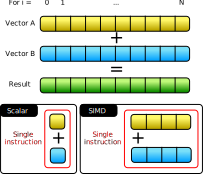
\includegraphics[width=\textwidth]{scalar_vs_SIMD.png}
        \end{column}
        \begin{column}{0.5\linewidth}
            \begin{itemize}
                \item Modern CPUs have instructions capable of doing multiple computations at the same time (e.g. do 4 distinct additions with a single instruction)
                \item SIMD: \highlight{S}ingle \highlight{I}nstruction \highlight{M}ultiple \highlight{D}ata
                \item Can get up to $N$ times faster with SIMD units of size $N$
            \end{itemize}
        \end{column}
    \end{columns}
\end{frame}

\begin{frame}[fragile]{What is vectorization}
    \begin{itemize}
        \item To vectorize, we use special functions called \highlight{intrinsics}
        \item These are functions provided by the compiler
        \item They map to hardware instructions
        \item SIMD intrinsics are only portable between CPUs using the same instruction set:
        \begin{itemize}
            \item x86 $\rightarrow$ SSE, AVX
            \item ARM $\rightarrow$ NEON, SVE
            \item RISC-V $\rightarrow$ RVV
            \item ...
        \end{itemize}
    \end{itemize}
\end{frame}

\begin{frame}[fragile]{Example: usage of SIMD intrinsics}
    For example, adding two SIMD vectors of \texttt{double} using intrinsics:
    \begin{columns}
        \begin{column}{0.5\linewidth}
            \begin{center}
                \caption{Using AVX2 (Intel, AMD CPUs)}
                \begin{minted}{C++}
                    #include <immintrin.h>

                    __m256d a, b;
                    a = _mm256_add_pd(a, b);
                \end{minted}
            \end{center}
        \end{column}
        \begin{column}{0.5\linewidth}
            \begin{center}
                \caption{Using SVE (ARM CPUs)}
                \begin{minted}{C++}
                    #include <arm_sve.h>

                    svfloat64_t a, b;
                    a = svadd_m(svptrue_b64(), a, b);
                \end{minted}
            \end{center}
        \end{column}
    \end{columns}

    \vspace{10pt}

    We run into \highlight{two problems}:
    \begin{enumerate}
        \item Writing code using intrinsics is not portable
        \item Writing code for each instruction set is repetitive and time-consuming
    \end{enumerate}
\end{frame}

\begin{frame}[fragile]{What about auto-vectorization?}
    \begin{columns}
        \begin{column}{0.5\linewidth}
            \begin{itemize}
                \item With the right flags, compilers can vectorize some parts of your code
                \item Not a solution to our problem, since vectorization is not guaranteed
                \item Sometimes the code is too complex for the compiler to vectorize (aliasing, dependencies, ...)
                \item \texttt{\#pragma ivdep} or \texttt{\#pragma omp simd} can help, but we cannot put pragmas on a Kokkos parallel loop
            \end{itemize}
        \end{column}
        \begin{column}{0.5\linewidth}
            \begin{minted}{C++}
                #pragma ivdep
                for (int i = 0; i < m; i++)
                    a[i] = a[i + k] * c;
            \end{minted}
            \begin{minted}{C++}
                Kokkos::parallel_for("loop", m,
                    KOKKOS_LAMBDA(int i) {
                        a(i) = a(i + k) * c;
                    });
            \end{minted}
        \end{column}
    \end{columns}
\end{frame}

\begin{frame}[fragile]{Vectorization libraries}
    \structure{Solution:} vectorization libraries

    \vspace{10pt}

    They offer:
    \begin{itemize}
        \item Higher level types and functions to manipulate vectors
        \item A C++ API to the SIMD intrinsics
        \item A portable abstraction over the platform specific intrinsics
    \end{itemize}
\end{frame}

\begin{frame}[fragile]{Vectorization libraries: Kokkos SIMD}
    \begin{columns}
        \begin{column}{0.4\linewidth}
            Kokkos comes with a vectorization library: \highlight{Kokkos SIMD}
            \begin{itemize}
                \item Specific header
                \item The platform specific vector type is abstracted away
                \item We use regular C++ operators to manipulate vectors
            \end{itemize}
        \end{column}
        \begin{column}{0.6\linewidth}
            \begin{center}
                \caption{AVX2}
                \begin{minted}{C++}
                    #include <immintrin.h>

                    __m256d a, b;
                    a = _mm256_add_pd(a, b);
                \end{minted}
            \end{center}
            \begin{center}
                \caption{Kokkos SIMD}
                \begin{minted}{C++}
                    #include <Kokkos_SIMD.hpp>

                    Kokkos::Experimental::simd<double> a, b;
                    a += b;
                \end{minted}
            \end{center}
        \end{column}
    \end{columns}
\end{frame}

\begin{frame}[fragile]{Vectorization libraries: C++ standard SIMD}
    \begin{itemize}
        \item The C++26 standard will include SIMD facilities
            \begin{minted}{C++}
                std::simd<double> x;
            \end{minted}
        \item Kokkos SIMD follows the same API
        \item It solves the portability between CPUs
        \item But Kokkos requires portability between CPU and GPU
        \item Using vectorized CPU instructions on the GPU is not possible \\
              We will see later how Kokkos handles this
    \end{itemize}
\end{frame}

\begin{frame}[fragile]{What Kokkos SIMD provides}
    \begin{itemize}
        \item A \texttt{Kokkos::Experimental::simd} type wrapping platform specific vectors
        \item A corresponding \texttt{Kokkos::Experimental::simd\_mask} type
        \item Operators for doing basic operations on these types (arithmetic, bitwise, shift, comparison, ...)
        \item No need to remember complicated intrinsics names
          \begin{minted}{C++}
              Kokkos::Experimental::simd<int> a, b, c;
              a *= (a + b) & (c << 2);
          \end{minted}
        \item Auxiliary functions (load, store, etc)
        \item Math functions working on SIMD types
    \end{itemize}
\end{frame}

\begin{frame}[fragile]{Kokkos SIMD}
    \begin{itemize}
        \item Kokkos SIMD supports the following datatypes: \texttt{float}, \texttt{double}, \texttt{int32\_t}, \texttt{uint32\_t}, \texttt{int64\_t}, \texttt{uint64\_t}
        \item \texttt{Kokkos::Experimental::simd<T>} will default to the vector type with the largest size for type \texttt{T}
        \item You can also explicitly request a size: \texttt{Kokkos::Experimental::simd<float, N>}\\
              Be careful, different platforms have different vector sizes
        \item If needed, you can also directly specify an abi: \texttt{Kokkos::Experimental::basic\_simd<float, abi>}
    \end{itemize}
    \begin{block}{SIMD abi}
        In Kokkos SIMD, abis are types used to identify an instruction set and a vector length. Using an abi directly is \highlight{not portable}.
    \end{block}
\end{frame}

\begin{frame}[fragile]{Supported SIMD abis}
    \begin{center}
        \begin{tblr}[theme=kokkostable]{lll}
        ISA & abi & Compatible datatypes \\
        - & \texttt{scalar} & all \\
        \SetCell[r=2]{c} AVX2 & \texttt{avx2\_fixed\_size<4>} & all \\
                              & \texttt{avx2\_fixed\_size<8>} & \texttt{float}, \texttt{int32\_t}, \texttt{uint32\_t} \\
        \SetCell[r=2]{c, bg=white} AVX512 & \texttt{avx512\_fixed\_size<8>} & all \\
                                & \texttt{avx512\_fixed\_size<16>} & \texttt{float}, \texttt{int32\_t}, \texttt{uint32\_t} \\
        \SetCell[r=2]{c} NEON & \texttt{neon\_fixed\_size<2>} & all \\
                              & \texttt{neon\_fixed\_size<4>} & \texttt{float}, \texttt{int32\_t}, \texttt{uint32\_t} \\
        \SetCell[r=2]{c, bg=white} SVE & \texttt{sve\_fixed\_size<N/2>} & \texttt{double}, \texttt{int64\_t}, \texttt{uint64\_t}, \texttt{int32\_t} \\
                             & \texttt{sve\_fixed\_size<N>} & \texttt{float}, \texttt{int32\_t}, \texttt{uint32\_t} \\
        \end{tblr}
    \end{center}
\end{frame}

\begin{frame}[fragile]{Initializing a vector}
    \begin{itemize}
        \item Default construction: the values will be uninitialized
            \vspace{-5pt}
            \begin{minted}{C++}
                Kokkos::Experimental::simd<double> x;
            \end{minted}
        \item Set every element to the same value
            \vspace{-5pt}
            \begin{minted}{C++}
                Kokkos::Experimental::simd<double> x(5.);
            \end{minted}
        \item Set each value individually
            \vspace{-5pt}
            \begin{minted}{C++}
                Kokkos::Experimental::simd<double> x(KOKKOS_LAMBDA(int idx) { return idx * idx; });
            \end{minted}
        \item Load the values from memory
            \vspace{-5pt}
            \begin{minted}{C++}
                Kokkos::Experimental::simd<double> x(ptr, Kokkos::Experimental::simd_flag_default);
            \end{minted}
    \end{itemize}
\end{frame}

\begin{frame}[fragile]{Vectorizing a loop}
    A loop typically has the following structure:
    \begin{minted}{C++}
        Kokkos::parallel_for("loop", N,
            KOKKOS_LAMBDA(int i) {
                // load input data
                // do some computation
                // store the result
            });
    \end{minted}

\end{frame}

\begin{frame}[fragile]{Vectorizing a loop}
    A vectorized loop follows the same pattern:
    \begin{minted}{C++}
        Kokkos::parallel_for("vectorized loop", N / VEC_WIDTH,
            KOKKOS_LAMBDA(int i) {
                // load input data into vectors
                // do some computation
                // store the result vector in memory
            });
    \end{minted}
    \structure{Note:} We iterate from 0 to \texttt{N / VEC\_WIDTH}, since we compute \texttt{VEC\_WIDTH} elements per iteration.
\end{frame}

\begin{frame}[fragile]{Example: adding two views}
    Let's start with a simple kernel adding two views
    \begin{minted}{C++}
        Kokkos::View<double*> A("A", N);
        Kokkos::View<double*> B("B", N);
        Kokkos::parallel_for("add", N,
            KOKKOS_LAMBDA(int i) {
                A(i) += B(i);
            }
        );
    \end{minted}
\end{frame}

\begin{frame}[fragile]{Example: adding two views}
    The vectorized version is as follows
    \begin{minted}{C++}
        Kokkos::View<double*> A("A", N);
        Kokkos::View<double*> B("B", N);
        using simd_type = Kokkos::Experimental::simd<double>;
        Kokkos::parallel_for("add", N / simd_type::size(),
            KOKKOS_LAMBDA(int i) {
                std::size_t idx = i * simd_type::size();
                // load the values
                simd_type a(&A(idx), Kokkos::Experimental::simd_flag_default);
                simd_type b(&B(idx), Kokkos::Experimental::simd_flag_default);
                // perform the computation
                a += b;
                // store the result
                Kokkos::Experimental::simd_unchecked_store(a, &A(idx), Kokkos::Experimental::simd_flag_default);
            });
    \end{minted}
\end{frame}

\begin{frame}[fragile]{Conditionals}
    \begin{itemize}
        \item Loops are not always simple
        \item Complex control flows can be problematic
            \begin{minted}{C++}
                Kokkos::parallel_for("loop", N,
                    KOKKOS_LAMBDA(int i) {
                        if (A(i) > 0)
                            A(i) = Kokkos::sqrt(A(i));
                        else
                            A(i) = 0;
                    });
            \end{minted}
        \item We cannot use an \texttt{if} branch with a vector
            \begin{itemize}
                \item Consider the following vector \texttt{\{-1, 2, 0, 1\}}
                \item Different values of the vector would enter different branches
                \item \structure{Solution:} the \texttt{condition} function, which selects values from two vectors according to a \highlight{mask}
            \end{itemize}
    \end{itemize}
\end{frame}

\begin{frame}[fragile]{Masks}
    \begin{itemize}
        \item \texttt{Kokkos::Experimental::simd\_mask} acts like a vector of booleans
        \item Initialized like a \texttt{simd} vector
            \begin{minted}{C++}
                using namespace Kokkos::Experimental;
                simd_mask<double> m;       // uninitialized
                simd_mask<double> m(true); // every value is true
                // true on even indices, false on odd ones
                simd_mask<double> m(KOKKOS_LAMBDA(int i) { return i % 2 == 0; });
            \end{minted}
        \item This is the type returned by comparison operations
            \begin{minted}{C++}
                Kokkos::Experimental::simd<double> x;
                Kokkos::Experimental::simd_mask<double> m = x > 0.;
            \end{minted}
        \item They can be used in the \texttt{condition} function, to conditionally load/store elements of a vector or in reduction operations
    \end{itemize}
\end{frame}

\begin{frame}[fragile]{Example: vectorizing with conditionals}
    Here is a kernel computing $a = \sqrt{a}$ if $a$ is positive, or $a = 0$ otherwise
    \begin{minted}{C++}
        Kokkos::View<double*> A("A", N);
        Kokkos::parallel_for("sqrt", N,
            KOKKOS_LAMBDA(int i) {
                if (A(i) > 0)
                    A(i) = Kokkos::sqrt(A(i));
                else
                    A(i) = 0.;
            }):
    \end{minted}
\end{frame}

\begin{frame}[fragile]{Example: vectorizing with conditionals}
    Here is the vectorized version
    \begin{minted}{C++}
        Kokkos::View<double*> A("A", N);
        using simd_type = Kokkos::Experimental::simd<double>;
        Kokkos::parallel_for("sqrt", N / simd_type::size(),
            KOKKOS_LAMBDA(int i) {
                std::size_t idx = i * simd_type::size();
                simd_type a(&A(idx), Kokkos::Experimental::simd_flag_default);
                a = condition(a > 0, Kokkos::sqrt(a), 0.);
                Kokkos::Experimental::simd_unchecked_store(a, &A(idx), Kokkos::Experimental::simd_flag_default);
            });
    \end{minted}
    \vspace{-10pt}
    \begin{itemize}
        \item \texttt{condition} takes a \texttt{simd\_mask}, and two vectors, and selects elements from both vectors depending on the values in the mask
        \item \structure{Note:} both branches are evaluated
    \end{itemize}
\end{frame}

\begin{frame}[fragile]{What about GPUs?}
    \begin{itemize}
    \item We said previously that we cannot use vectorized CPU instructions on GPU
    \item But we just used SIMD inside a \texttt{Kokkos::parallel\_for}
    \item To keep portability, we default to a scalar type when using a GPU backend
    \end{itemize}

    \begin{center}
        \begin{tblr}[theme=kokkostable]{colspec=lll, row{2}={bg=lightmain}}
            & \SetCell[c=2]{l} Kokkos compiled on \\
            SIMD alias & CPU backend & GPU backend \\
            \texttt{simd<T>} & \texttt{basic\_simd<T, abi<...>>} & \texttt{basic\_simd<T, scalar>} \\
            \texttt{simd<T, N>} & \texttt{basic\_simd<T, abi<N>>} & \texttt{basic\_simd<T, scalar>} \\
            \texttt{basic\_simd<T, abi<N>>} & \texttt{basic\_simd<T, abi<N>>} & \texttt{basic\_simd<T, abi<N>>} \\
        \end{tblr}
    \end{center}
\end{frame}

% _____________________________________________________________________________

\section{Debugging and profiling}

\begin{frame}{What is this about?}
    \begin{columns}[T]
        \begin{column}{0.5\linewidth}
            \begin{center}
                \textbf{Debugging}
            \end{center}
            \begin{itemize}
                \item Errors may happen
                \item Print-debugging is cumbersome
                \item Developers need real tools
                \begin{itemize}
                    \item \texttt{gdb} (CPU)
                    \item \texttt{compute-sanitizer} (Cuda)
                    \item \texttt{cuda-gdb} (Cuda)
                    \item ...
                \end{itemize}
                \item What can Kokkos do?
            \end{itemize}
        \end{column}
        \pause
        \begin{column}{0.5\linewidth}
            \begin{center}
                \textbf{Profiling}
            \end{center}
            \begin{itemize}
                \item You want to optimize real bottlenecks
                \item \texttt{time} has its limits
                \item You don't want to create timers by yourself
                \item Developers need real tools
                \begin{itemize}
                    \item \texttt{perf} (CPU)
                    \item VTune (CPU)
                    \item NSight Systems/Compute (Cuda)
                    \item ...
                \end{itemize}
                \item What can Kokkos do?
            \end{itemize}
        \end{column}
    \end{columns}
\end{frame}

\begin{frame}{Kokkos debugging and profiling tools at hand}
    \begin{columns}[T]
        \begin{column}{0.33\linewidth}
            \begin{center}
                \textbf{Kokkos}
            \end{center}
            \begin{itemize}
                \item KokkosP interface
                \item Profiling regions
            \end{itemize}
            \begin{block}{Note}
                Not actual tools, but used by other tools
            \end{block}
            \begin{block}{Remark}
                Same interface for debugging and profiling
            \end{block}
        \end{column}
        \pause
        \begin{column}{0.33\linewidth}
            \begin{center}
                \textbf{Kokkos tools}
            \end{center}
            \begin{itemize}
                \item Kernel logger
                \item Kernel timer
                \item Memory usage
                \item Memory events
                \item Space time stack
                \item VTune connector
                \item NVTX connector
                \item ROCTX connector
                \item ...
            \end{itemize}
        \end{column}
        \pause
        \begin{column}{0.33\linewidth}
            \begin{center}
                \textbf{Third-party tools}
            \end{center}
            \begin{itemize}
                \item VTune
                \item Nsight Systems
                \item Nsight Compute
                \item Tau
                \item Timemory
                \item Caliper
                \item HPCToolkit
                \item Apex
                \item ...
            \end{itemize}
        \end{column}
    \end{columns}
\end{frame}

\begin{frame}[fragile]{KokkosP interface}
    \begin{columns}
        \begin{column}{0.55\linewidth}
            \begin{minted}{C++}
                Kokkos::View<int *> view("view", N);

                Kokkos::parallel_for(
                    "compute",
                    N,
                    KOKKOS_LAMBDA(int i) {
                        view(i) = // ...
                    }
                );

                Kokkos::fence(
                    "wait for compute"
                );
            \end{minted}
        \end{column}
        \begin{column}{0.45\linewidth}
            \begin{itemize}
                \item Profiling tools interface
                \item Provided by Kokkos
                \item Hooks in Kokkos functions
                \begin{itemize}
                    \item Parallel constructs
                    \item Fences
                \end{itemize}
                \item Designed for other tools to use it
                \item Always available
                \item Really small overhead if no tools are used (check of a Boolean)
            \end{itemize}
        \end{column}
    \end{columns}
\end{frame}

\begin{frame}[fragile]{Profiling regions}
    \begin{columns}
        \begin{column}{0.5\linewidth}
            \begin{minted}{C++}
                Kokkos::Profiling::pushRegion(
                    "computation"
                );

                // ...

                Kokkos::Profiling::popRegion();
            \end{minted}
        \end{column}
        \begin{column}{0.5\linewidth}
            \begin{itemize}
                \item Provided by Kokkos
                \item No specific header needed
                \item Namespace \texttt{Kokkos::Profiling}
                \item Set regions of interest in your code
                \begin{itemize}
                    \item \texttt{pushRegion} to create a region
                    \item \texttt{popRegion} to remove a region
                \end{itemize}
                \item Regions can be nested
            \end{itemize}
        \end{column}
    \end{columns}
\end{frame}

\begin{frame}{Kokkos tools}
    \begin{itemize}
        \item Library of the Kokkos ecosystem
        \item \githublink{\url{https://github.com/kokkos/kokkos-tools}}
        \item \doclink{\url{https://github.com/kokkos/kokkos-tools/wiki}}
        \item Has a different version number than Kokkos
        \item Should be built and installed somewhere (this requires to install Kokkos too)
        \item Use one tool at a time with the environment variable \texttt{KOKKOS\_TOOLS\_LIBS}

        Mind the \texttt{S}!
        \item Do not ship it within your program (this is a dev tool!)
    \end{itemize}
\end{frame}

\begin{frame}[fragile]{Guided tour for a dummy code}
    \begin{columns}
        \begin{column}{0.6\linewidth}
           \begin{minted}[fontsize=\scriptsize]{C++}
                Kokkos::Profiling::pushRegion("computation");

                Kokkos::View<int *> view("view", N);

                Kokkos::parallel_for(
                    "compute",
                    N,
                    KOKKOS_LAMBDA(int i) {
                        view(i) = i;
                    }
                );

                Kokkos::fence("wait for compute");

                Kokkos::Profiling::popRegion();
            \end{minted}
        \end{column}
        \begin{column}{0.4\linewidth}
            \begin{itemize}
                \item Very simple code
                \item Let's try some tools on it
            \end{itemize}
        \end{column}
    \end{columns}
\end{frame}

\begin{frame}[fragile]{Simple kernel logger for a basic debugging}
    \begin{columns}
        \begin{column}{0.6\linewidth}
            \begin{minted}[breakafter=/]{sh}
                export KOKKOS_TOOLS_LIBS=/absolute/path/to/libkp_kernel_logger.so

                ./my_program
            \end{minted}

            \begin{minted}{text}
                KokkosP: Kernel Logger Library Initialized (sequence is 0, version: 20240906)
            \end{minted}
        \end{column}
        \begin{column}{0.4\linewidth}
            \begin{itemize}
                \item Simple tool for a basic logging of your program's Kokkos-related activity
                \item Export environment variable to use the tool
                \item Run the program as usual
                \item Run for a few number of iterations if possible
                \item When loaded, a tool always print something on screen
            \end{itemize}
        \end{column}
    \end{columns}
\end{frame}

\begin{frame}[fragile]{Simple kernel logger output}
    \begin{minted}[fontsize=\tiny]{text}
        KokkosP: Entering profiling region: computation
        KokkosP: Allocate<Cuda> name: view pointer: 0x7c67126aa000 size: 80000
        KokkosP: Executing fence on device 33554433 with unique execution identifier 0
        KokkosP: computation
        KokkosP:       SharedAllocationRecord<Kokkos::CudaSpace, void>::SharedAllocationRecord(): fence after copying header from HostSpace
        KokkosP: Execution of fence 0 is completed.
        KokkosP: Executing parallel-for kernel on device 33554433 with unique execution identifier 1
        KokkosP: computation
        KokkosP:       Kokkos::View::initialization [view] via memset
        KokkosP: Execution of kernel 1 is completed.
        KokkosP: Executing fence on device 33554433 with unique execution identifier 2
        KokkosP: computation

        ...

        KokkosP: Kokkos library finalization called.
    \end{minted}

    \begin{itemize}
        \item All Kokkos activity listed (parallel constructs, fences, View creations...)
        \item Useful for tracking chaining of kernels
        \item Difficult to read for long executions or when the kernels are asynchronous
        \item Good idea to redirect the output to a file
    \end{itemize}
\end{frame}

\begin{frame}[fragile]{Simple kernel timer for a basic profiling}
    \begin{columns}
        \begin{column}{0.6\linewidth}
            \begin{minted}[breakafter=/]{sh}
                export KOKKOS_TOOLS_LIBS=/absolute/path/to/libkp_kernel_timer.so

                ./my_program
            \end{minted}

            \usemintedstyle{vim}
            \begin{minted}{text}
                KokkosP: Simple Kernel Timer Library Initialized (sequence is 0, version: 20240906)
                ...
                KokkosP: Kernel timing written to /path/to/name_of_report.dat
            \end{minted}

            \begin{minted}{sh}
                kp_reader ./name_of_report.dat
            \end{minted}
        \end{column}
        \begin{column}{0.4\linewidth}
            \begin{itemize}
                \item Simple tool for a basic timing analysis
                \item Export environment variable to use the tool
                \item Run the program as usual
                \item Analyze the generated data with the provided \texttt{kp\_reader} program
            \end{itemize}
        \end{column}
    \end{columns}
\end{frame}

\begin{frame}[fragile]{Simple kernel timer output}
    \begin{minted}{text}
         (Type)   Total Time, Call Count, Avg. Time per Call, %Total Time in Kernels, %Total Program Time
        -------------------------------------------------------------------------
        Regions:
        ...
        -------------------------------------------------------------------------
        Kernels:
        ...
        -------------------------------------------------------------------------
        Summary:
        ...
        -------------------------------------------------------------------------
    \end{minted}
    \begin{itemize}
        \item 3 sections in the report
        \item Let's analyze them
    \end{itemize}
\end{frame}

\begin{frame}[fragile]{Simple kernel timer output (for summary)}
    \begin{minted}{text}
         (Type)   Total Time, Call Count, Avg. Time per Call, %Total Time in Kernels, %Total Program Time
        -------------------------------------------------------------------------
        Summary:

        Total Execution Time (incl. Kokkos + non-Kokkos):                   0.00038 seconds
        Total Time in Kokkos kernels:                                       0.00030 seconds
        -> Time outside Kokkos kernels:                                  0.00008 seconds
        -> Percentage in Kokkos kernels:                                   78.75 %
        Total Calls to Kokkos Kernels:                                            2

        -------------------------------------------------------------------------
    \end{minted}
    \begin{itemize}
        \item Global metrics of the execution of the program
        \item Example for a very simple code
    \end{itemize}
\end{frame}

\begin{frame}[fragile]{Simple kernel timer output (for regions)}
    \begin{minted}{text}
         (Type)   Total Time, Call Count, Avg. Time per Call, %Total Time in Kernels, %Total Program Time
        -------------------------------------------------------------------------

        Regions:

        - computation
        (REGION)   0.000349 1 0.000349 117.590361 92.599620
    \end{minted}

    \begin{itemize}
    	\item Regions are named after what you set in \texttt{pushRegion}
        \item Descending order of cumulated duration
    	\item One set of two lines per region
    \end{itemize}
\end{frame}

\begin{frame}[fragile]{Simple kernel timer output (for kernels)}
    \begin{minted}{text}
         (Type)   Total Time, Call Count, Avg. Time per Call, %Total Time in Kernels, %Total Program Time

        -------------------------------------------------------------------------
        Kernels:

        - compute
        (ParFor)   0.000282 1 0.000282 94.939759 74.762808
        - Kokkos::View::initialization [view] via memset
        (ParFor)   0.000015 1 0.000015 5.060241 3.984820
    \end{minted}

    \begin{itemize}
	    \item Kernels are named after what you set in parallel constructs (\texttt{parallel\_*})
        \item Some internal kernels are visible: Views initialization
        \item Descending order of cumulated duration
	    \item One set of two lines per kernel
    \end{itemize}
\end{frame}

\begin{frame}{NVTX connector for NVIDIA tools}
    \begin{itemize}
        \item Simple connector to convert Kokkos named regions/kernels into NVTX regions
        \item NVIDIA Tools eXtension
        \item For NVIDIA tools
        \begin{itemize}
            \item Nsight Systems
            \item Nsight Compute
        \end{itemize}
        \item Lot of documentation about how to use these tools right
        \item Equivalent ROCTX connector for AMD
    \end{itemize}
\end{frame}

\begin{frame}[fragile]{NVTX connector and Nsight Systems}
    \begin{columns}
        \begin{column}{0.6\linewidth}
            \begin{minted}[breakafter=/]{sh}
                export KOKKOS_TOOLS_LIBS=/absolute/path/to/libkp_nvtx_connector.so

                nsys profile \
                    -o report \
                    ./my_program
                nsys-ui report.nsys-rep
            \end{minted}

            \begin{minted}{text}
                KokkosP: NVTX Analyzer Connector (sequence is 0, version: 20240906)
            \end{minted}
        \end{column}
        \begin{column}{0.4\linewidth}
            \begin{itemize}
                \item Analyze a program as a whole
                \item Export environment variable to use the tool
                \item Run the program through \texttt{nsys}
                \item Do not run your program for too long when profiling!
                \item About 10 iterations is enough
                \item Open the generated report
            \end{itemize}
        \end{column}
    \end{columns}
\end{frame}

\begin{frame}{Nsight Systems overview}
    \begin{columns}
        \begin{column}{0.75\linewidth}
            \includegraphics[width=\linewidth]{nsight_systems_example}
        \end{column}
        \begin{column}{0.25\linewidth}
            \begin{itemize}
                \item Activity against execution time
                \item Cuda activity
                \begin{itemize}
                    \item Kernels
                    \item Memory
                \end{itemize}
                \item NVTX
                \begin{itemize}
                    \item Parallel constructs
                    \item Fences
                    \item Regions
                \end{itemize}
                \item Cuda API calls
            \end{itemize}
        \end{column}
    \end{columns}
\end{frame}

\begin{frame}{Display NVTX name of kernels in Nsight Systems}
    \begin{columns}
        \begin{column}{0.5\linewidth}
            \begin{itemize}
                \item Kernels are named after function name, which for Kokkos is an obscure internal name
                \item Set to rename the kernels after the NVTX name
                \begin{enumerate}
                    \item Tools $\rightarrow$ Options
                    \item Behavior $\rightarrow$ Report
                    \item Set "Rename CUDA Kernels by NVTX" to \emph{Yes}
                    \item Re-open the report
                \end{enumerate}
            \end{itemize}
        \end{column}
        \begin{column}{0.5\linewidth}
            \includegraphics[width=\linewidth]{nsight_systems_options}
        \end{column}
    \end{columns}
\end{frame}

\begin{frame}[fragile]{NVTX connector and Nsight Compute}
    \begin{columns}
        \begin{column}{0.6\linewidth}
            \begin{minted}[breakafter=/]{sh}
                export KOKKOS_TOOLS_LIBS=/absolute/path/to/libkp_nvtx_connector.so

                ncu \
                    -o report \
                    --nvtx \
                    --nvtx-include "<NVTX region>/" \
                    --set detailed \
                    ./my_program
                ncu-ui report.ncu-rep
            \end{minted}

            \begin{minted}{text}
                KokkosP: NVTX Analyzer Connector (sequence is 0, version: 20240906)
            \end{minted}
        \end{column}
        \begin{column}{0.4\linewidth}
            \begin{itemize}
                \item Kernel by kernel analysis
                \item Export environment variable to use the tool
                \item Run the program through \texttt{ncu}
                \item Use NVTX region to profile only certain kernels
                \item Set of metrics to collect
                \item The more the metrics, the slower the profiling
                \item Run for about 10 iterations
                \item Open the generated report
            \end{itemize}
        \end{column}
    \end{columns}
\end{frame}

\begin{frame}{Nsight Compute overview}
    \begin{columns}
        \begin{column}{0.75\linewidth}
            \includegraphics[width=\linewidth]{nsight_compute_example}
        \end{column}
        \begin{column}{0.25\linewidth}
            \begin{itemize}
                \item Details of each kernel
                \item Many metrics
                \begin{itemize}
                    \item Speed of light
                    \item Occupancy
                    \item ...
                \end{itemize}
                \item Can give suggestions
                \item Check online resources!
            \end{itemize}
        \end{column}
    \end{columns}
\end{frame}

\begin{exerciseframe}{Exercise 10: Profiling a Kokkos program}
    \begin{columns}
        \begin{column}{0.5\linewidth}
            \begin{center}
                
\includegraphics[width=0.9\textwidth]{sleeping_otter.png}
            \end{center}

            Go to the exercise \githublink{\href{https://github.com/CExA-project/cexa-kokkos-tutorials/tree/main/exercises/10_profiling}{10\_profiling}} and follow the instructions
        \end{column}
        \begin{column}{0.5\linewidth}
            \begin{block}{Goal of this exercise}
                \begin{itemize}
                    \item Use Kokkos profiling regions
                    \item Use meaningful labels in parallel constructs and fences
                    \item Debug with the simple kernel timer
                    \item Profile with the simple kernel logger
                    \item Profile with Nsight Systems
                    \item Profile with Nsight Compute
                \end{itemize}
            \end{block}
        \end{column}
    \end{columns}
\end{exerciseframe}

\section{Conclusion}

\begin{frame}{Conclusion}
    Congratulation, you have learned intermediate notions of Kokkos!

    \begin{itemize}
        \item How and why to use atomic operations
        \item How to use SIMDs
        \item How to debug and profile a Kokkos program
    \end{itemize}
\end{frame}

\end{document}
